\documentclass[10pt]{beamer}

%\setbeameroption{show notes on second screen=right}

% -------------------- Theme --------------------
\usetheme{Madrid}
%\setbeamertemplate{navigation symbols}{}

\setbeamercovered{transparent}

% -------------------- Ahmedabad University Colors --------------------
\definecolor{AUred}{RGB}{128,18,20}      % Primary logo red
\definecolor{AUdark}{RGB}{160,160,160}    % Dark gray for text
\definecolor{AUlight}{RGB}{242,239,236} % Light background


\definecolor{arsenic}{rgb}{0.23, 0.27, 0.29}
\definecolor{bole}{rgb}{0.47, 0.27, 0.23}
\definecolor{brown(web)}{rgb}{0.65, 0.16, 0.16}
\definecolor{cadet}{rgb}{0.33, 0.41, 0.47}
\definecolor{cordovan}{rgb}{0.54, 0.25, 0.27}
\definecolor{daffodil}{rgb}{1.0, 1.0, 0.19}
\definecolor{brown(traditional)}{rgb}{0.59, 0.29, 0.0}
\colorlet{slidebg}{white}
\colorlet{boxbg}{blue!6}
\colorlet{textlight}{black}
\colorlet{netblue}{blue!65!black}
\colorlet{embedgreen}{green!45!black}
\colorlet{SharedWeight}{red!60!black}
\colorlet{distamber}{orange!80!black}

% -------------------- Apply Colors --------------------
\setbeamercolor{structure}{fg=AUred}

\setbeamercolor{title}{fg=AUlight}
\setbeamercolor{subtitle}{fg=AUdark}

\setbeamercolor{frametitle}{fg=AUdark, bg=AUred}
\setbeamercolor{framesubtitle}{fg=AUlight}
\setbeamercolor{section in head/foot}{fg=AUlight, bg=AUred}

\setbeamercolor{block title}{fg=AUlight, bg=AUred}
\setbeamercolor{block body}{fg=black, bg=AUlight}

\setbeamercolor{item}{fg=AUred}
\setbeamercolor{subitem}{fg=AUred}

\setbeamercolor{footline}{fg=white, bg=AUred}

% -------------------- Frame Title Fonts --------------------
\setbeamerfont{frametitle}{size=\small,series=\bfseries}
\setbeamerfont{framesubtitle}{size=\large}

\setbeamerfont{caption}{size=\scriptsize}


% -------------------- Packages --------------------
\usepackage{amsmath}
\usepackage{amsfonts}
\usepackage{graphicx}
\usepackage{booktabs}
\usepackage{nameref}
\usepackage{natbib}
\usepackage{tikz}
\usepackage{amssymb}    % for \checkmark
\usepackage{multirow}


\usetikzlibrary{calc, positioning, arrows.meta, fit, backgrounds, shapes.geometric}
\usepackage{xcolor}
\bibliographystyle{plainnat}





% Local colors (already defined in preamble via color_fix — kept here for safety)
\providecolor{netblue}{named}{blue}
\colorlet{SBlue}{blue!70!black}
\colorlet{SGreen}{green!50!black}
\colorlet{SRed}{red!60!black}
\colorlet{SAmber}{orange!85!black}
\colorlet{SBlueBg}{blue!9}
\colorlet{SGreenBg}{green!9}
\colorlet{SRedBg}{red!8}
\colorlet{SAmberBg}{orange!10}
\colorlet{SGrayBg}{black!5}



% -------------------- Title Info --------------------
\title[Online Tracker for Small Object Detection]{Improve performance of existing online trackers for small object detection}
\subtitle{UAV videos}

\author[Sheth A., Parekh M., Thanki K., Riddhi B.]{
	Team Name: \textbf{The Convolutioners} \\
	\textbf{Aagam Sheth} (AU2544006) \\	
	\textbf{Mahima Parekh} (AU2544003) \\
	\textbf{Khevan Thanki} (AU23L20002) \\
	\textbf{Riddhi Bhargava} (AU2220028)
}

\institute[]{
	Instructor Name: \textbf{Prof. Mehul Raval} \\
	Assigned TA: \textbf{Daksh D. Shah} \\
	School of Engineering and Applied Science \\
	\vspace{0.2cm}
	\includegraphics[width=3cm]{"/home/aagamsheth/Documents/Education/Ahmedabad University/media/au_logo.png"}
}

\date{\today}

% -------------------- Logo on Each Slide --------------------
\addtobeamertemplate{frametitle}{}{
	\hfill
	\raisebox{0.7cm}[0pt][0pt]{\includegraphics[height=0.8cm,keepaspectratio]{"/home/aagamsheth/Documents/Education/Ahmedabad University/media/au_logo_dark.png"}}
}


% -------------------- Document --------------------
\begin{document}
	
	% -------------------- Title Slide --------------------
	{
		% \logo{}
		\begin{frame}
			\titlepage
		\end{frame}
	}
	
	\begin{frame}{Background}{Problem Statement}	
		\begin{itemize}
			\item \textbf{Challenges} faced in detection:
				\begin{itemize}
					\item Tiny objects $\rightarrow$ few pixels
					\item Clutter, motion blur, scale variation
					\item Unreliable detections
				\end{itemize}
		\end{itemize}
		
		\vspace{0.25cm}
		\begin{itemize}
			\item Unreliable detections lead to:
			\begin{itemize}
				\item Missed detections
				\item Identity switches
				\item Poor tracking performance
			\end{itemize}
		\end{itemize}
		
		\vspace{0.5cm}
		\begin{block}{Research Gap}
			Existing methods are not optimized for small object detection in UAV scenarios, resulting in poor detection quality and inconsistent identity association even with tiling and ReID.
		\end{block}
	\end{frame}

    % --------------------------------------------------------
    \begin{frame}{Small Object Detection \& Tracking}{Literature Review}
    	\begin{columns}[T]
    		\begin{column}{0.48\textwidth}
    			\textbf{Spatial Detection Challenges}
    			\begin{itemize}
    				\scriptsize
    				\item \textbf{UAV Constraints:} High altitude and scale variance render standard CNN receptive fields inadequate.
    				\item \textbf{Architectural Evolution:} Feature Pyramid Networks (FPN) and YOLO11 leverage multi-scale semantic merging.
    				\item \textbf{Tiling (SAHI):} Image slicing prevents downsampling loss, preserving high-resolution features for small targets.
    			\end{itemize}
    		\end{column}
    		
    		\begin{column}{0.48\textwidth}
    			\textbf{Temporal Tracking \& Re-ID}
    			\begin{itemize}
    				\scriptsize
    				\item \textbf{Association:} Occlusions and crowds necessitate Siamese-based Re-Identification (Re-ID).
    				\item \textbf{Metric Learning:} Contrastive and Focal-BCE losses optimize distance-based embedding discrimination.
    				\item \textbf{Optimization:} Optuna (TPE) replaces grid search for efficient Bayesian hyperparameter tuning.
    			\end{itemize}
    		\end{column}
    	\end{columns}
    	
    	\vspace{0.4cm}
    	\begin{block}{The Proposed Pipeline}
    		\centering \footnotesize
    		\textbf{SAHI + Fine-tuned YOLO11 + Optimized Siamese Re-ID + BoT-SORT}
    	\end{block}
    \end{frame}


    % ----------------------------------------------------------
    



    % -----------------------------------------------------------

	\begin{frame}{Full pipeline of work}{Methodology Overview}
		\centering
		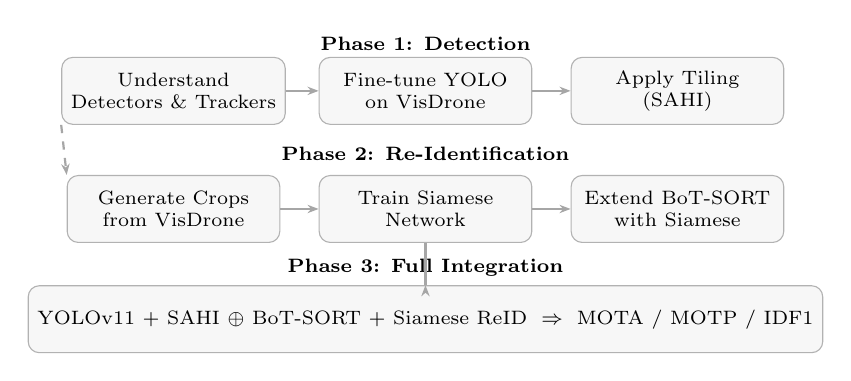
\begin{tikzpicture}[
			>=Stealth,
			box/.style={
				draw=black!30, fill=black!3, rounded corners=4pt,
				minimum width=2.7cm, minimum height=0.85cm,
				align=center, font=\scriptsize
			},
			arr/.style={-{Stealth[length=4pt]}, line width=0.8pt, color=black!35},
			]
			
			% ── Phase 1 ──────────────────────────────────────────────────────
			\node[font=\scriptsize\bfseries, draw=none] at (3.2, 2.3) {Phase 1: Detection};
			
			\node[box] (n1) at (0,   1.7) {Understand\\Detectors \& Trackers};
			\node[box] (n2) at (3.2, 1.7) {Fine-tune YOLO\\on VisDrone};
			\node[box] (n3) at (6.4, 1.7) {Apply Tiling\\(SAHI)};
			
			\draw[arr] (n1) -- (n2);
			\draw[arr] (n2) -- (n3);
			
			% ── Phase 2 ──────────────────────────────────────────────────────
			\node[font=\scriptsize\bfseries, draw=none] at (3.2, 0.9) {Phase 2: Re-Identification};
			
			\node[box] (p1) at (0,   0.2) {Generate Crops\\from VisDrone};
			\node[box] (p2) at (3.2, 0.2) {Train Siamese\\Network};
			\node[box] (p3) at (6.4, 0.2) {Extend BoT-SORT\\with Siamese};
			
			\draw[arr] (p1) -- (p2);
			\draw[arr] (p2) -- (p3);
			\draw[arr, dashed] (n1.south west) -- (p1.north west);
			
			% ── Phase 3 ──────────────────────────────────────────────────────
			\node[font=\scriptsize\bfseries, draw=none] at (3.2, -0.55) {Phase 3: Full Integration};
			
			\node[box, minimum width=9cm] (final) at (3.2, -1.2)
			{YOLOv11 + SAHI $\oplus$ BoT-SORT + Siamese ReID
				$\;\Rightarrow\;$ MOTA / MOTP / IDF1};
			
			\draw[arr] (p2.south) -- ++(0,-0.1) |- (final.north);
			
		\end{tikzpicture}
	\end{frame}
	
	\begin{frame}{Results}{Baseline Metrics}
		\footnotesize
		\definecolor{good}{RGB}{0,140,0}
		\definecolor{bad}{RGB}{200,0,0}
		
		\begin{table}
			\centering
			\setlength{\tabcolsep}{5pt}
			\begin{tabular}{lcccc}
				\toprule
				\textbf{Metric} & \textbf{YOLOv8n} & \textbf{YOLO11} & \textbf{YOLO11} & \textbf{YOLO11 + SAHI} \\
				& \textbf{(Siamese NW)} & \textbf{(FT)}   & \textbf{+ SAHI} & \textbf{+ BotSort} \\
				&                       &                 &                 & \textbf{(380, 0.3)} \\
				\midrule
				MOTA      & 0.129                                 & 0.1673                  & 0.1728                  & \textcolor{bad}{0.0740}          \\
				IDF1      & 0.224                                 & \textcolor{good}{0.4902}& 0.4879                  & 0.4382                            \\
				HOTA      & \textcolor{good}{0.260}               & 0.2124                  & --                      & --                                \\
				DetA      & 0.142                                 & \textcolor{good}{0.3014}& --                      & --                                \\
				AssA      & \textcolor{good}{0.504}               & 0.1557                  & --                      & --                                \\
				MOTP      & 0.222                                 & 0.2651                  & \textcolor{good}{0.2601}& 0.2578                            \\
				Precision & \textcolor{good}{0.8168}              & --                      & 0.6112                  & 0.5491                            \\
				Recall    & 0.1298                                & --                      & 0.4907                  & \textcolor{good}{0.4456}          \\
				FPS       & \textcolor{good}{12.69}               & 0.5                     & 0.5                     & --                                \\
				\bottomrule
			\end{tabular}
		\end{table}	
	\end{frame}
	
	
	\begin{frame}{Results}{Siamese Network Analysis}
		\footnotesize
		\centering
		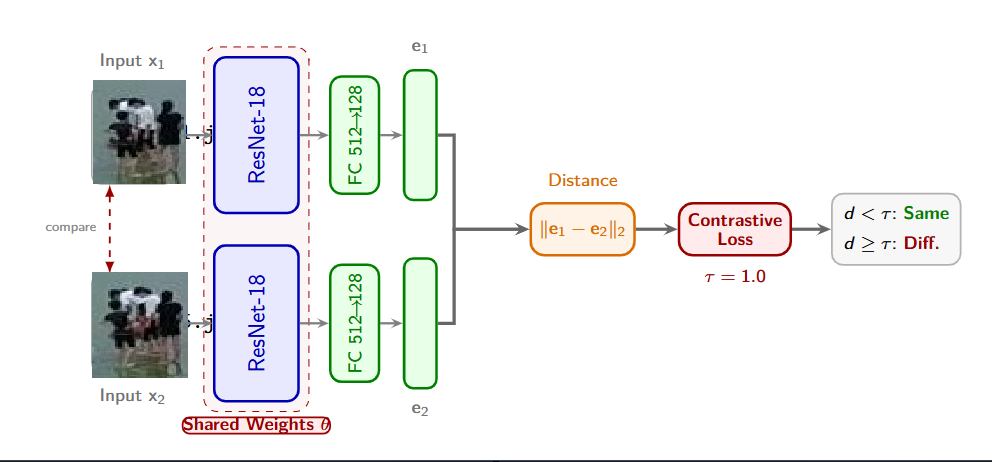
\includegraphics[width=\textwidth]{3.png}
	\end{frame}



    \begin{frame}{Siamese Network}{Grid Sweep Optimisation}
    \begin{columns}[T]
        \begin{column}{0.45\textwidth}
            \textbf{Key Findings:}
            \begin{itemize}
                \small
                \item \textbf{Best Model (Run 12):} ResNet18 ($d=64$, $m=1.2$) achieved \textbf{0.989 F1} with high discriminative separation ($\approx 20.6\times$ distance ratio).
                \item \textbf{End-to-End Training:} Freezing backbones (Run 4) dropped F1 to 0.829; fine-tuning is vital for UAV imagery.
                \item \textbf{Efficiency:} ResNet18 matched ResNet34 accuracy but trained \textbf{2.4$\times$ faster}, making it the optimal real-time choice.
            \end{itemize}
        \end{column}

        \begin{column}{0.52\textwidth}
            \begin{table}
                \scriptsize
                \centering
                \caption{Top-5 Grid Sweep Runs}
                \label{tab:grid_sweep}
                \begin{tabular}{llccc}
                    \toprule
                    Run & Backbone & $d$ & $m$ & F1 \\
                    \midrule
                    12 & ResNet18        & 64  & 1.2 & \textbf{0.989} \\
                    10 & ResNet34        & 64  & 0.8 & 0.988 \\
                    1  & MobileNetV3-S   & 256 & 0.8 & 0.964 \\
                    5  & ResNet18        & 256 & 1.0 & 0.906 \\
                    4  & ResNet18$^{*}$  & 64  & 1.2 & 0.829 \\
                    \bottomrule
                \end{tabular}
                \vspace{1mm}
                \begin{flushleft}
                    \tiny $^{*}$Frozen backbone. All others unfrozen with L2 norm.
                \end{flushleft}
            \end{table}
        \end{column}
    \end{columns}
\end{frame}
    
	
	
	
	\begin{frame}{Siamese Network Training}{Initial Baseline vs. Optimised Configuration}
    \begin{table}[h]
        \centering
        \label{tab:siamese_comparison}
        \setlength{\tabcolsep}{6pt}
        
        % --- Baseline ---
        \textbf{(a) Baseline (MobileNetV3-S, $d=256$, lr=$10^{-4}$, $m=1.0$)}
        \vspace{0.15cm}
        
        \begin{tabular}{cccccc}
        \toprule
        Epoch & Loss & Acc & Prec & Rec & F1 \\
        \midrule
        1 & 2.660 & 0.660 & 0.600 & 0.970 & 0.740 \\
        2 & 0.210 & 0.670 & 0.610 & 0.990 & 0.750 \\
        3 & 0.130 & 0.710 & 0.630 & 1.000 & 0.770 \\
        4 & 0.090 & \textbf{0.790} & 0.700 & 1.000 & \textbf{0.820} \\
        5 & \textbf{0.080} & 0.770 & 0.680 & 1.000 & 0.810 \\
        \bottomrule
        \end{tabular}
        
        \vspace{0.2cm}
        
        % --- Optimised ---
        \textbf{(b) Optimised (ResNet18, $d=64$, lr=$3\times10^{-4}$, $m=1.2$, L2 norm)}
        \vspace{0.1cm}
        
        \begin{tabular}{cccccc}
        \toprule
        Epoch & Loss & Acc & Prec & Rec & F1 \\
        \midrule
        1 & 0.071 & 0.993 & 0.991 & 0.995 & 0.993 \\
        2 & 0.030 & 0.992 & 0.988 & 0.996 & 0.992 \\
        3 & 0.024 & 0.994 & 0.988 & 0.999 & 0.994 \\
        4 & 0.021 & 0.996 & 0.995 & 0.997 & 0.996 \\
        5 & \textbf{0.017} & \textbf{0.997} & 0.994 & \textbf{1.000} & \textbf{0.997} \\
        \bottomrule
        \end{tabular}
        
        \vspace{0.3cm}
        \raggedright
        \small\textit{Bold values indicate best per-column result within each configuration.
        The optimised model achieves F1\,=\,0.997 vs.\ 0.820 for the baseline --- a gain of
        $+0.177$ --- with loss converging $4.7\times$ lower by epoch 5.}
        
        \end{table}

    \end{frame}

\begin{frame}{Training dynamics}{Optimised Siamese network}
	\footnotesize
	\centering
	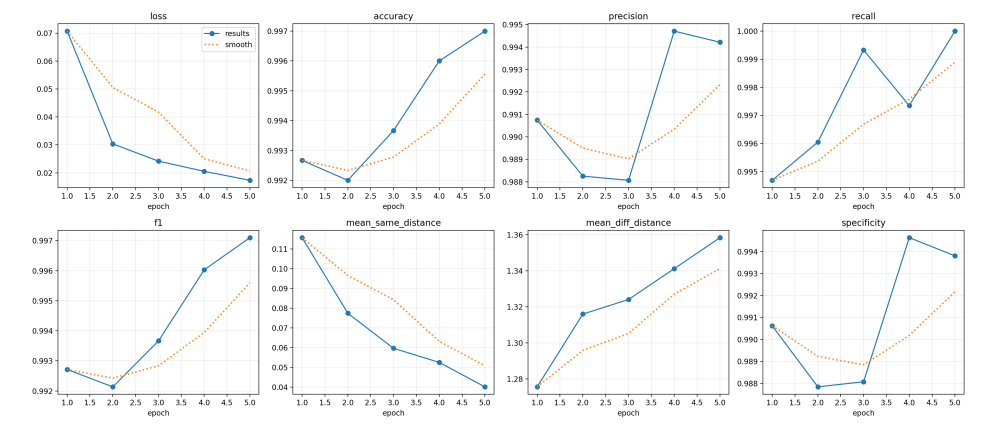
\includegraphics[width=\textwidth]{training_metrics.png}
\end{frame}

\begin{frame}{Training dynamics}{Same vs Different Object Distance}
	\footnotesize
	\centering
	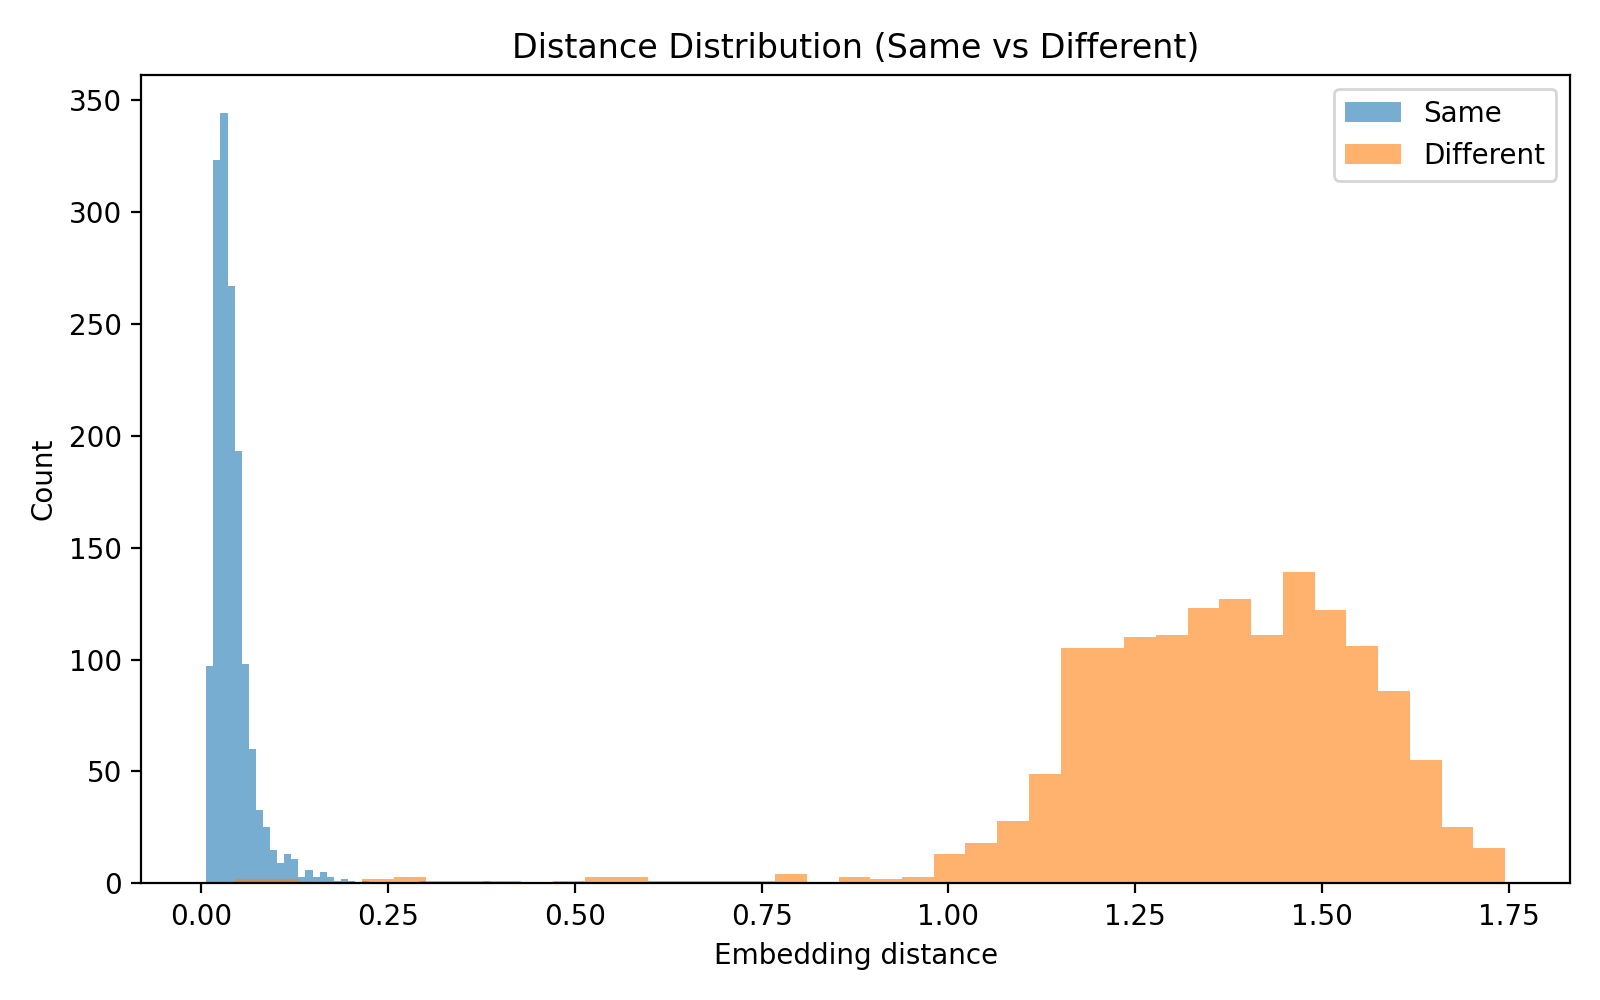
\includegraphics[width=\textwidth]{distance_histogram.png}
\end{frame}



\begin{frame}{Siamese Network}{Hyperparameter \& Threshold Analysis}
    \begin{columns}[T]
        % Left Column: Threshold Sweep
        \begin{column}{0.48\textwidth}
            \centering
            \textbf{Distance Threshold ($\tau$) Sweep}
            \vspace{0.2cm}
            \begin{table}
                \scriptsize
                \centering
                \begin{tabular}{ccccc}
                    \toprule
                    $\tau$ & Acc & Prec & Recall & F1 \\
                    \midrule
                    0.5 & 0.784 & \textbf{0.838} & 0.693 & 0.759 \\
                    0.8 & 0.776 & 0.740 & 0.851 & 0.791 \\
                    1.0 & 0.762 & 0.690 & 0.916 & \textbf{0.802} \\
                    1.2 & 0.706 & 0.632 & 0.959 & 0.762 \\
                    1.5 & 0.517 & 0.500 & 0.995 & 0.666 \\
                    \bottomrule
                \end{tabular}
            \end{table}
            \begin{itemize}
                \tiny
                \item \textbf{High Precision:} $\tau=0.5$ minimizes false ID matches.
                \item \textbf{Optimal F1:} $\tau=1.0$ provides the best overall balance.
                \item \textbf{Saturation:} $\tau > 1.5$ leads to random-guess precision.
            \end{itemize}
        \end{column}

        % Visual Divider
        \vrule{}

        % Right Column: Optuna Results
        \begin{column}{0.48\textwidth}
            \centering
            \textbf{Optuna Bayesian Optimization}
            \vspace{0.2cm}
            \begin{table}
                \scriptsize
                \centering
                \begin{tabular}{ccccc}
                    \toprule
                    Trial & $d$ & $w_{\text{neg}}$ & L2 & F1 \\
                    \midrule
                    \textbf{7} & 64 & 2.03 & No & \textbf{0.844} \\
                    2 & 64 & 2.31 & Yes & 0.843 \\
                    8 & 64 & 2.60 & Yes & 0.835 \\
                    6 & 128 & 2.26 & Yes & 0.792 \\
                    0 & 128 & 2.81 & Yes & 0.786 \\
                    \bottomrule
                \end{tabular}
            \end{table}
            \begin{itemize}
                \tiny
                \item \textbf{Best Settings:} Focal-BCE with $w_{\text{neg}} \approx 2.0$ and $d=64$.
                \item \textbf{Backbone:} End-to-end fine-tuning consistently outperformed frozen backbones.
                \item \textbf{L2 Norm:} Top trial succeeded without L2 normalization.
            \end{itemize}
        \end{column}
    \end{columns}
\end{frame}


\begin{frame}{Siamese Network}{Alternative Loss Comparison}
    \begin{itemize}
        \item \textbf{Objective:} Compare standard Focal-BCE (\textit{Baseline}) against a precision-weighted variant (\textit{Enhanced}) to minimize identity switches in tracking.
    \end{itemize}

    \begin{table}
        \small
        \centering
        \caption{Focal-BCE Variant Comparison (5 Epochs)}
        \label{tab:loss_comparison}
        \begin{tabular}{lcccccc}
            \toprule
            Variant & $w_{\text{neg}}$ & Acc & Prec & Recall & F1 & \textbf{FP} \\
            \midrule
            Baseline & 1.0 & 0.787 & 0.709 & \textbf{0.964} & 0.817 & 586 \\
            Enhanced FP-Red & 2.0 & \textbf{0.808} & \textbf{0.753} & 0.924 & \textbf{0.830} & \textbf{460} \\
            \bottomrule
        \end{tabular}
    \end{table}

    \vspace{2mm}

    \begin{columns}[T]
        \begin{column}{0.48\textwidth}
            \begin{block}{Enhanced Advantage}
                \begin{itemize}
                    \scriptsize
                    \item \textbf{False Positive Reduction:} Dropped from 586 to 460 (\textbf{$-21.5\%$}).
                    \item \textbf{Improved Precision:} Increased to 0.753, crucial for reducing spurious track initializations.
                \end{itemize}
            \end{block}
        \end{column}
        
        \begin{column}{0.48\textwidth}
            \begin{block}{The Trade-off}
                \begin{itemize}
                    \scriptsize
                    \item \textbf{False Negatives:} Increased from 53 to 115 as the model becomes more "conservative."
                    \item \textbf{Verdict:} Enhanced variant is preferred for BoT-SORT integration to protect \textbf{MOTA} scores.
                \end{itemize}
            \end{block}
        \end{column}
    \end{columns}
\end{frame}



\begin{frame}{BoT-SORT Tracker}{Full Benchmark Results}
    \begin{itemize}
        \item \textbf{Comparison:} Baseline YOLO11 vs. SAHI-tiled inference across 7 validation sequences.
    \end{itemize}

    \begin{table}
        \scriptsize
        \centering
        \caption{Pipeline Comparison (VisDrone2019-MOT Val)}
        \label{tab:pipeline_global}
        \begin{tabular}{lccc}
            \toprule
            \textbf{Metric} & Prelim. (CPU) & \textbf{YOLO+Siamese} & SAHI+Siamese \\
            \midrule
            \textbf{MOTA} $\uparrow$ & 0.129 & \textbf{0.326} & 0.061 \\
            IDF1 $\uparrow$ & 0.224 & \textbf{0.504} & 0.453 \\
            HOTA@0.5 $\uparrow$ & 0.260 & \textbf{0.495} & 0.429 \\
            AssA@0.5 $\uparrow$ & 0.504 & \textbf{0.629} & 0.532 \\
            \midrule
            \textbf{FP} $\downarrow$ & 35,629 & \textbf{11,374} & 52,478 \\
            \textbf{ID Switches} $\downarrow$ & 657 & \textbf{578} & 1,405 \\
            \midrule
            \textbf{FPS} $\uparrow$ & 12.69 & 5.84 & 1.27 \\
            \bottomrule
        \end{tabular}
    \end{table}

    \begin{block}{Key Observation}
        \small
        While SAHI is intended for small objects, it introduced a massive surge in \textbf{False Positives (FP)} and \textbf{ID Switches}, leading to a significant MOTA degradation compared to the standard YOLO11-fine-tuned pipeline.
    \end{block}
\end{frame}


% -----------------------------------------------------------------------

% add the phases metrics 




% -------------------------------------------------------------------------



\begin{frame}{BoT-Sort Tracker}{BoT-SORT Hyperparameter Tuning}
	
	\textbf{Goal}
	\begin{itemize}
		\item Systematically improve tracking performance using a 4-phase tuning strategy
	\end{itemize}
	
	\textbf{Evaluation Strategy}
	\begin{itemize}
		\item All trials logged for reproducibility
		\item Composite score:
		\begin{itemize}
			\item 0.45 $\times$ IDF1
			\item 0.35 $\times$ HOTA
			\item 0.20 $\times$ MOTA
		\end{itemize}
		\item Focus: identity consistency
	\end{itemize}
	
	\textbf{Phase 1: Association Tuning (10 trials)}
	\begin{itemize}
		\item Parameters: appearance\_weight, match\_cost\_thresh, IoU thresholds
		\item Best configuration:
		\begin{itemize}
			\item appearance\_weight = 0.65
			\item match\_cost\_thresh = 0.72
		\end{itemize}
		\item Key finding: Optimal balance between appearance and spatial matching achieved at these values
	\end{itemize}
	
\end{frame}



\begin{frame}{BoT-Sort Tracker}{Lifecycle Tuning}
	
	\textbf{Phase 2: Track Lifecycle (24 trials)}
	\begin{itemize}
		\item Parameters: min\_hits, max\_age, new\_track\_thresh
		\item Key finding: min\_hits = 1 is optimal since UAV objects appear briefly and require immediate track confirmation
	\end{itemize}
	
	\textbf{Phase 3: Kalman Filter (Pending)}
	\begin{itemize}
		\item Tune motion model and noise parameters
	\end{itemize}
	
	\textbf{Phase 4: Reassociation (Pending)}
	\begin{itemize}
		\item Recover lost tracks
		\item Reduce fragmentation
	\end{itemize}
	
\end{frame}




\begin{frame}{Detailed Performance}{YOLO vs. SAHI Comparison}
    \centering

    \begin{itemize}
        \item \textbf{CMC Integration:} Sparse optical flow CMC implemented to mitigate UAV ego-motion and inflate IoU accuracy.
        \item \textbf{Optimization Progress:} 
        \begin{itemize}
            \item \textbf{Phases 1--2 (Complete):} Calibration of gates/lifecycle; \texttt{min\_hits=1} identified as critical.
            \item \textbf{Phases 3--4 (Pending):} Kalman dynamics and local reassociation remain incomplete.
        \end{itemize}
    \end{itemize}
    \small \textbf{Per-Sequence MOTA / IDF1 / HOTA Breakdown}
    \vspace{0.1cm}

    \begin{table}
        \renewcommand{\arraystretch}{1.1}
        \fontsize{7.5pt}{8.5pt}\selectfont
        \centering
        \begin{tabular}{l | ccc | ccc}
            \toprule
            & \multicolumn{3}{c|}{\textbf{YOLO11 + Siamese (Ours)}} & \multicolumn{3}{c}{\textbf{SAHI + Siamese}} \\
            \textbf{Sequence ID} & \textbf{MOTA} $\uparrow$ & \textbf{IDF1} $\uparrow$ & \textbf{HOTA} $\uparrow$ & \textbf{MOTA} & \textbf{IDF1} & \textbf{HOTA} \\
            \midrule
            uav0000086 & 0.361 & 0.512 & 0.469 & 0.295 & 0.499 & 0.446 \\
            uav0000117 & 0.280 & 0.473 & 0.474 & \color{red}{-0.532} & 0.348 & 0.360 \\
            uav0000137 & 0.367 & 0.539 & 0.515 & 0.165 & 0.494 & 0.421 \\
            uav0000182 & 0.324 & 0.526 & 0.485 & 0.158 & 0.507 & 0.447 \\
            uav0000268 & 0.150 & 0.270 & 0.318 & 0.018 & 0.267 & 0.313 \\
            uav0000305 & \textbf{0.512} & \textbf{0.705} & \textbf{0.682} & \color{red}{-0.056} & 0.565 & 0.560 \\
            uav0000339 & 0.348 & 0.509 & 0.522 & 0.221 & 0.469 & 0.454 \\
            \midrule
            \textbf{Overall} & \textbf{0.326} & \textbf{0.504} & \textbf{0.495} & 0.061 & 0.453 & 0.429 \\
            \bottomrule
        \end{tabular}
    \end{table}

    \vspace{0.2cm}

\end{frame}





% ---------------------------------------------------------





% -------------------------------------------------------


    
    	
	\begin{frame}{Future Scope}{Refining the Existing Pipeline}
 
\begin{table}
\centering
\footnotesize
\renewcommand{\arraystretch}{1.1}
\begin{tabular}{@{}p{2.0cm} p{6.4cm} p{3.0cm}@{}}
\toprule
\textbf{Component} & \textbf{Refinement} & \textbf{Expected gain} \\
\midrule
 
\textbf{SAHI tiling}\newline\footnotesize{(detection)}
  & Per-sequence tiling policy: sweep slice size $\{384,512,640\}$ $\times$ overlap $\{0.2,0.3,0.4\}$; class-aware NMM threshold (tighter for cars, looser for pedestrians); edge-padded slices to avoid boundary truncation.
  & Recall $\uparrow$ on 20--40\,px objects;\newline fewer boundary fragments \\
 
\textbf{Siamese ReID + NMS}\newline\footnotesize{(appearance)}
  & \textbf{Embedding-aware NMS}: before tracker input, suppress duplicate boxes whose cosine-sim $> \tau_e$ \emph{and} IoU $> \tau_i$ (survives a bbox-only NMS collision). Temperature-scale embeddings; L2-normalise before cache write.
  & Fewer duplicate tracks;\newline cleaner ID assignment \\
 
\textbf{BotSort hyperparams}\newline\footnotesize{(association)}
  & Grid-search on val:
  \texttt{track\_high}$\in\{0.5, 0.6\}$,
  \texttt{new\_track}$\in\{0.6, 0.7\}$,
  \texttt{match}$\in\{0.7, 0.8\}$,
  \texttt{appearance}$\in\{0.2, 0.25\}$,
  \texttt{proximity}$\in\{0.4, 0.5\}$,
  \texttt{buffer}$\in\{30, 45, 60\}$;
  CMC warp $\to$ affine \emph{before} predict (not after).
  & MOTA $\uparrow$, IDs $\downarrow$,\newline IDF1 $\uparrow$ \\
 
\bottomrule
\end{tabular}
\end{table}
  
\end{frame}



    % ------------------------------------------------

    
	

    % -----------------------------------------------
	
	\begin{frame}{Appendix}{References}
		
		\footnotesize
		
		\begin{itemize}
			
			\item Xiao, Y. et al. (2025). \textit{UAV video vehicle detection: Benchmark and baseline}. IEEE TGRS.
			
			\item Wang, J. et al. (2021). \textit{Tiny object detection in aerial images}. ICPR.
			
			\item Liu, M. et al. (2020). \textit{UAV-YOLO: Small object detection from UAV perspective}. Sensors.
			
			\item Feng, F. et al. (2024). \textit{Improved YOLOv8 for small object detection in aerial imagery}. Journal of King Saud University.
			
		\end{itemize}
		
	\end{frame}




    
	
	
\end{document}